%
% Modified by Megan Patnott
% Last Change: Jan 18, 2013
%
%%%%%%%%%%%%%%%%%%%%%%%%%%%%%%%%%%%%%%%%%%%%%%%%%%%%%%%%%%%%%%%%%%%%%%%%
%
% Modified by Sameer Vijay
% Last Change: Tue Jul 26 2005 13:00 CEST
%
%%%%%%%%%%%%%%%%%%%%%%%%%%%%%%%%%%%%%%%%%%%%%%%%%%%%%%%%%%%%%%%%%%%%%%%%
%
% Sample Notre Dame Thesis/Dissertation
% Using Donald Peterson's ndthesis classfile
%
% Written by Jeff Squyres and Don Peterson
%
% Provided by the Information Technology Committee of
%   the Graduate Student Union
%   http://www.gsu.nd.edu/
%
% Nothing in this document is serious except the format.  :-)
%
% If you have any suggestions, comments, questions, please send e-mail
% to: ndthesis@gsu.nd.edu
%
%%%%%%%%%%%%%%%%%%%%%%%%%%%%%%%%%%%%%%%%%%%%%%%%%%%%%%%%%%%%%%%%%%%%%%%%


%
% Chapter 3
%

\chapter{EXPERIMENTAL APPARATUS}

\section{The Large Hadron Collider}
The most powerful machine of its kind, the Large Hadron
Collider (LHC) accelerates and collides particles
at high center-of-mass energies producing rare
particles and interactions that would be otherwise unobservable
in the laboratory, making it the best tool available for studying \tth
processes. The LHC is a circular particle accelerator/collider. Measuring 27 km
in circumference, it collides beams of protons in head-on collisions       
at a center-of-mass energy of 13 TeV.

The LHC itself is technically the final element in a series of machines
that accelerate the beams from rest to succesively higher energies. This system of
of accelerators, referred to as the LHC Accelerator Complex is depicted below in
Figure~\ref{fig:lhc_complex}.

The acceleration is accomplished with radio frequency
(RF) cavities. RF cavities are a linear series of cylindrical conductors,
which sustain a resonant electromagnetic field produced by a generator. As 
charged particles pass through the cavities, they experience a force
(acceleration) from the resonant alternating field in each cavity.

This acceleration process begins with Hydrogen gas in the linear accelerator
(LINAC 2). The Hydrogen atoms in the gas are stripped of electrons
in an applied electric field, leaving only protons, which are then accelerated
along the linear beam pipe with RF cavities to an energy of 50 MeV. 

After the LINAC, the beams of protons enter the Proton Synchrontron Booster rings where
they are accelerated to 1.4 GeV, before reaching the Proton
Synchrotron (PS). The circular PS, measuring more than 600 m
in circumference, accelerates the beams to 25 GeV before injection into the
larger, Super Proton Synchrotron (SPS). The SPS at over 7 km around, provides the final
acceleration before the beams reach the LHC at an energy 450 GeV. The SPS injects the beams into
the LHC in opposite directions.

As a result of the RF cavity acceleration, the beams are comprised of independent
trains of 'bunches' of protons. 
 

After the beams are fully injected, the LHC ramps the beam energy to 6.5 TeV per beam,
providing 13 TeV center-of-mass proton collisions. 

\begin{figure}[hbtp]
 \begin{center}
   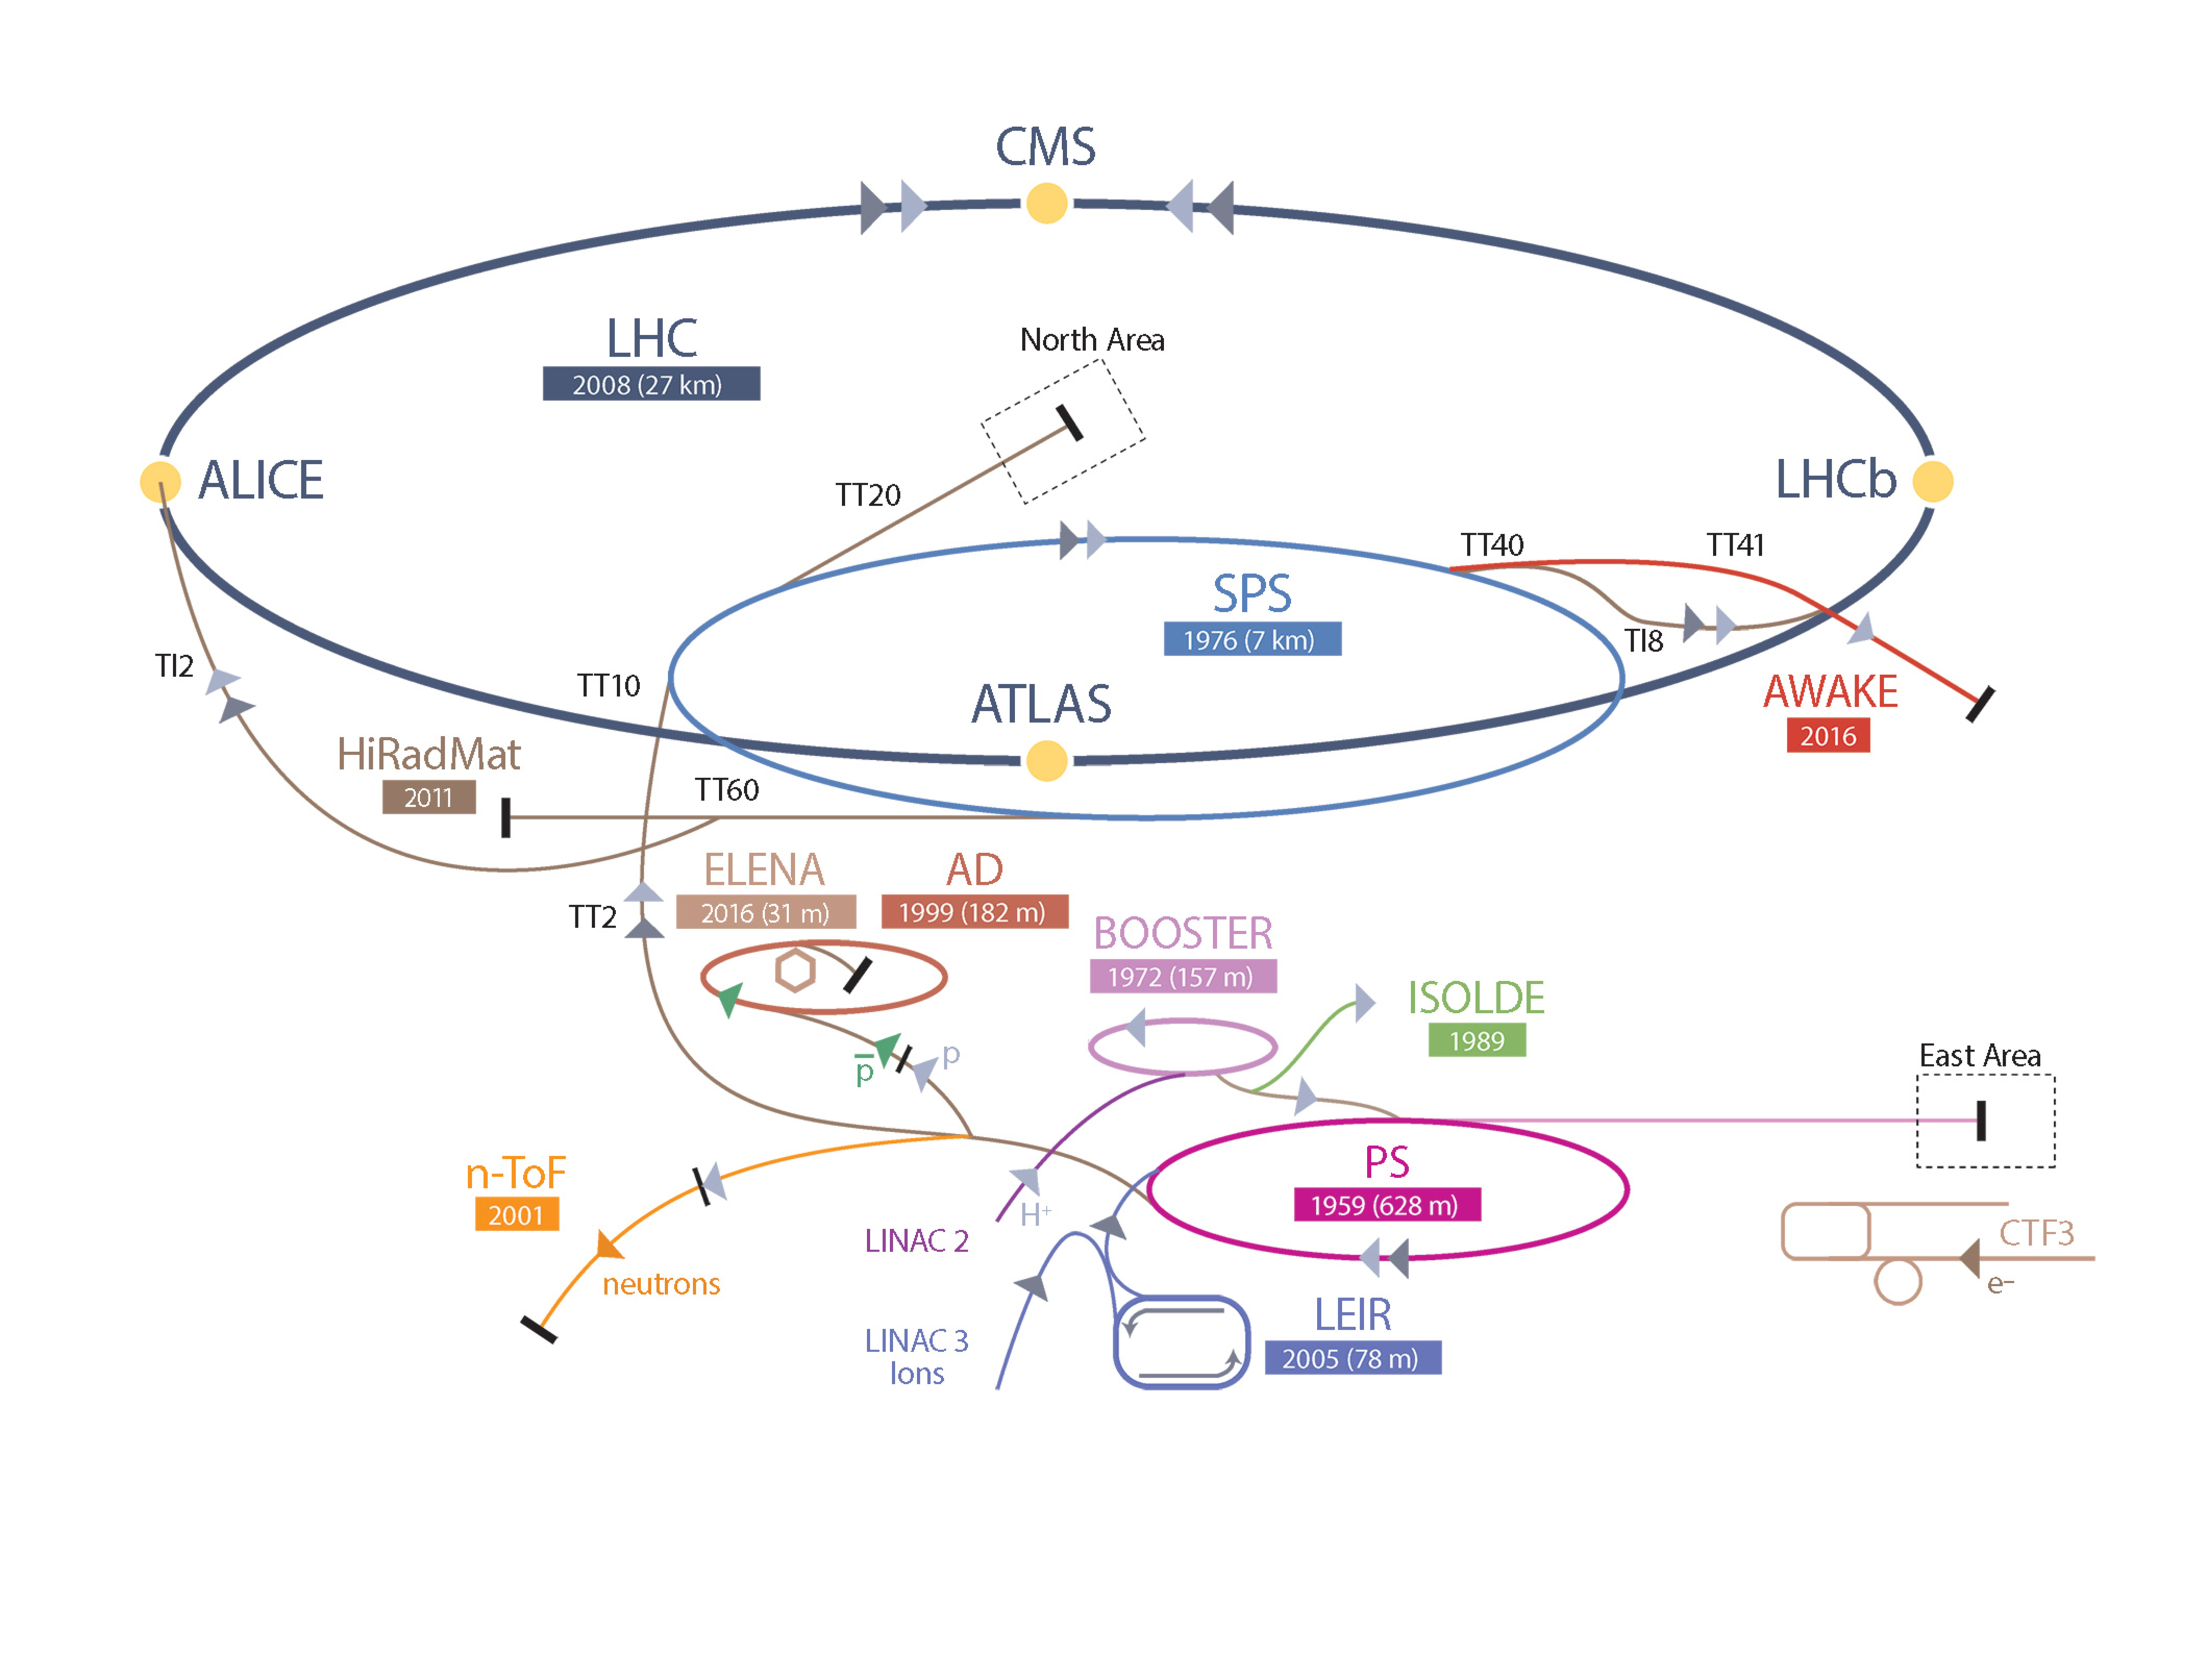
\includegraphics[width=0.9\textwidth]{lhc_complex.pdf}
   \caption[text in square brackets]{text in curly brackets}
   \label{fig:lhc_complex}
 \end{center}
\end{figure}

Inside the LHC, the beams travel in opposite directions in separate pipes adjacent to
one another. The beam pipes of the entire accelerator complex are kept at an ultra high vaccuum
to avoid detrimental beam interactions before the collisions. The beams are focused
and guided around the LHC with 392 quadrupole and 1232 dipole superconducting
magnets respectively.

The magnets produce a field of over 8 Tesla. This is accomplished via superconducting 
niobium-titanium coils. Cooled with liquid nitrogren and superfluid helium-4, these
magnets operate at 1.9 K and carry a current of over 11000 amperes. In addition to
the LHC, these magnets are used throughout the accelerator complex.

\section{The Compact Muon Solenoid (CMS) Detector}
This is an overview of the introduction.  In here, I will use many
many buzzwords and other legalistic-types of terms, mostly beginning on
the expounding of the holistic and synergistic energy that Gnus bring
to our organizations. If you offer some food, they will take it and back off a
respectful distance in order to consume their food while leaving you
to your ``personal space.''  

% % uncomment the following lines,
% if using chapter-wise bibliography
%
% \bibliographystyle{ndnatbib}
% \bibliography{example}
